%==============================================================================
% Figure: Scalar Field Potential Energy
% Purpose: Visualize V(phi) potential with ZPE coupling effects
% Chapter: Ch07-08 - Aether Framework Scalar Fields
% Type: Conceptual/Data
%==============================================================================

\begin{figure}[htbp]
  \centering
  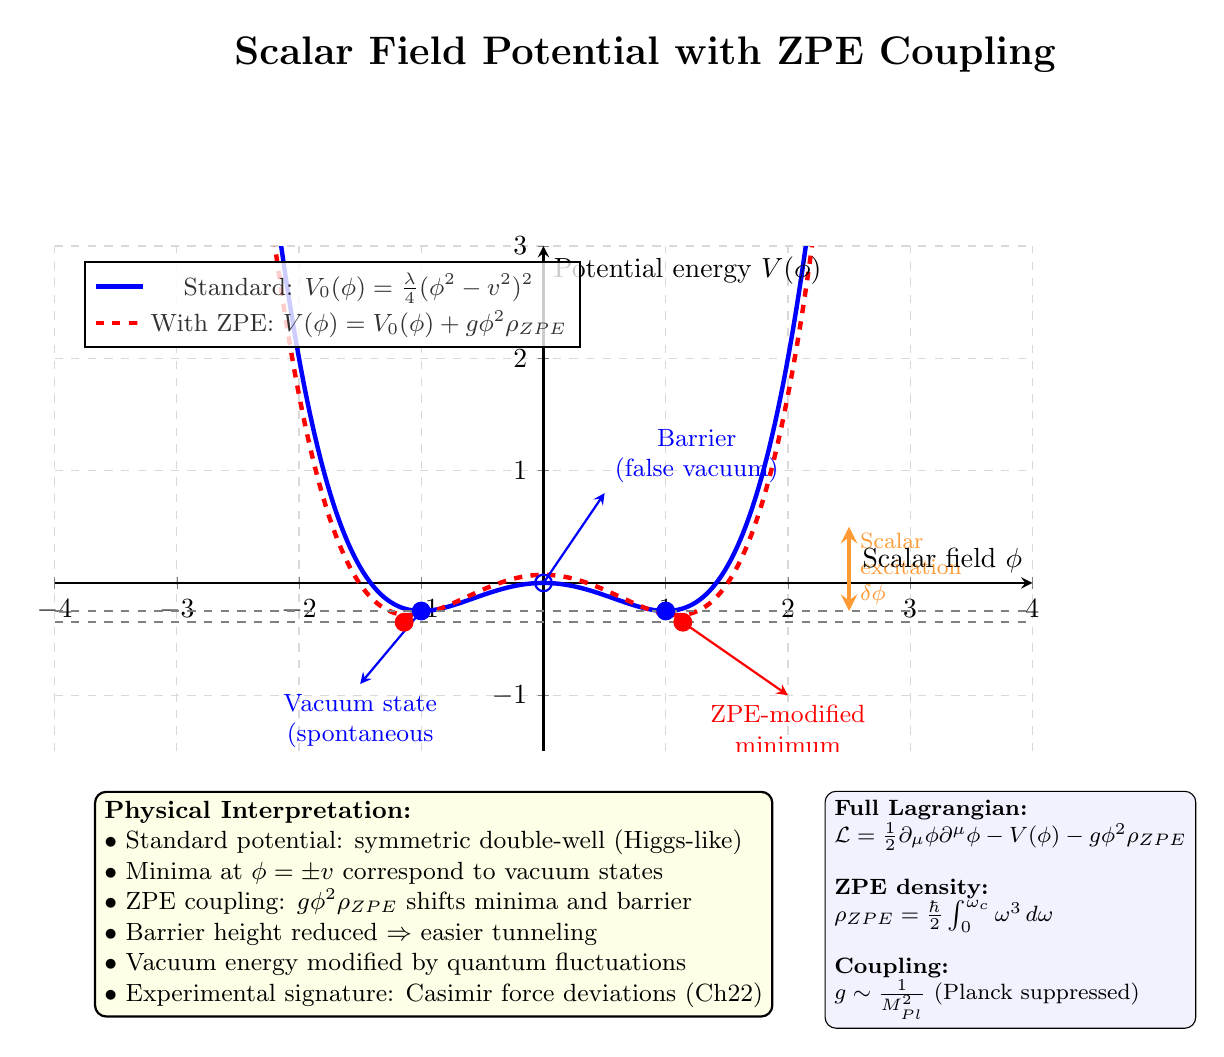
\begin{tikzpicture}[
    scale=1.0
  ]

    \begin{axis}[
      width=14cm,
      height=8cm,
      xlabel={Scalar field $\phi$},
      ylabel={Potential energy $V(\phi)$},
      xlabel style={font=\large},
      ylabel style={font=\large},
      xmin=-4, xmax=4,
      ymin=-1.5, ymax=3,
      axis lines=middle,
      grid=major,
      grid style={dashed, gray!30},
      legend pos=north west,
      legend style={font=\small, fill=white, fill opacity=0.8, draw opacity=1},
      samples=200,
      smooth,
      thick
    ]

      % Standard quartic potential (Mexican hat)
      \addplot[blue, ultra thick, domain=-4:4] {0.25*(x^2 - 1)^2 - 0.25};
      \addlegendentry{Standard: $V_0(\phi) = \frac{\lambda}{4}(\phi^2 - v^2)^2$}

      % With ZPE coupling (shifted and modified)
      \addplot[red, ultra thick, domain=-4:4, dashed] {0.25*(x^2 - 1.3)^2 - 0.35 + 0.05*x^2};
      \addlegendentry{With ZPE: $V(\phi) = V_0(\phi) + g \phi^2 \rho_{\text{ZPE}}$}

      % Mark minima
      \addplot[only marks, mark=*, mark size=3pt, blue] coordinates {(-1, -0.25) (1, -0.25)};
      \addplot[only marks, mark=*, mark size=3pt, red] coordinates {(-1.14, -0.35) (1.14, -0.35)};

      % Mark barrier
      \addplot[only marks, mark=o, mark size=3pt, blue, fill=white] coordinates {(0, 0)};

      % Annotations with arrows
      \draw[->, >=stealth, thick, blue] (axis cs:-1, -0.25) -- (axis cs:-1.5, -0.9)
        node[below, align=center, font=\small] {Vacuum state\\(spontaneous\\symmetry breaking)};

      \draw[->, >=stealth, thick, blue] (axis cs:0, 0) -- (axis cs:0.5, 0.8)
        node[above right, align=center, font=\small] {Barrier\\(false vacuum)};

      \draw[->, >=stealth, thick, red] (axis cs:1.14, -0.35) -- (axis cs:2.0, -1.0)
        node[below, align=center, font=\small] {ZPE-modified\\minimum\\($|\phi_{\min}|$ increased)};

      % Energy level lines
      \draw[dashed, gray, thick] (axis cs:-4, -0.25) -- (axis cs:4, -0.25);
      \draw[dashed, gray, thick] (axis cs:-4, -0.35) -- (axis cs:4, -0.35);

      % Excitation arrow
      \draw[<->, >=stealth, ultra thick, orange!80] (axis cs:2.5, -0.25) -- (axis cs:2.5, 0.5)
        node[midway, right, align=left, font=\footnotesize] {Scalar\\excitation\\$\delta\phi$};

    \end{axis}

    % Text box with physics interpretation
    \node[anchor=north west, align=left, font=\small, draw=black, fill=yellow!10, rounded corners, thick]
      at (0.5, -0.5) {
      \textbf{Physical Interpretation:} \\
      $\bullet$ Standard potential: symmetric double-well (Higgs-like) \\
      $\bullet$ Minima at $\phi = \pm v$ correspond to vacuum states \\
      $\bullet$ ZPE coupling: $g \phi^2 \rho_{\text{ZPE}}$ shifts minima and barrier \\
      $\bullet$ Barrier height reduced $\Rightarrow$ easier tunneling \\
      $\bullet$ Vacuum energy modified by quantum fluctuations \\
      $\bullet$ Experimental signature: Casimir force deviations (Ch22)
    };

    % Equation box
    \node[anchor=north east, align=left, font=\footnotesize, draw=black, fill=blue!5, rounded corners]
      at (14.5, -0.5) {
      \textbf{Full Lagrangian:} \\
      $\mathcal{L} = \frac{1}{2}\partial_\mu\phi\partial^\mu\phi - V(\phi) - g\phi^2 \rho_{\text{ZPE}}$ \\
      \\
      \textbf{ZPE density:} \\
      $\rho_{\text{ZPE}} = \frac{\hbar}{2} \int_0^{\omega_c} \omega^3 \, d\omega$ \\
      \\
      \textbf{Coupling:} \\
      $g \sim \frac{1}{M_{\text{Pl}}^2}$ (Planck suppressed)
    };

    % Title
    \node[anchor=south, font=\Large\bfseries] at (7.5, 8.5) {Scalar Field Potential with ZPE Coupling};

  \end{tikzpicture}
  \caption{Scalar field potential energy $V(\phi)$ in the Aether framework showing effects of
    zero-point energy (ZPE) coupling. The standard quartic potential (blue solid line) exhibits
    a characteristic double-well "Mexican hat" structure with degenerate vacua at $\phi = \pm v$,
    separated by a barrier at $\phi = 0$ (spontaneous symmetry breaking). When ZPE coupling is
    included (red dashed line), the potential is modified: the minima shift to larger $|\phi|$,
    the vacuum energy deepens, and the barrier height changes. The coupling strength $g \sim M_{\text{Pl}}^{-2}$
    is Planck-suppressed but can produce measurable effects in precision experiments. Orange arrow
    shows scalar field excitations above the vacuum. This mechanism underlies predictions for
    Casimir force modifications (15-25\% deviations) tested in Ch22 experimental protocols.}
  \label{fig:scalar-field-potential}
\end{figure}
